\chapter{Algorytmy i struktury danych}
\PartialToc
Autorzy odpowiedzi: Wojciech Kasperek, Wojciech Kryściński
Dla ułatwienia odpowiedzi będziemy podpisywać inicjałami.

\section{Które stwierdzenia spośród poniższych są prawdziwe} 

\vspace{0.4cm}
\noindent \textbf{Proponowana dpowiedź:} Pesymistyczna i oczekiwana złożoność obliczeniowa są sobie równe dla sortowania przez wybieranie. \\ 
\noindent \textbf{Odpowiedź:} Pesymistyczna i oczekiwana złożoność obliczeniowa są sobie równe dla sortowania przez wybieranie. \\ 
\noindent \textbf{Wyjaśnienie:}
\begin{center}
	\begin{tabular}{ | l | l | l | l |}
		\hline
		Algorytm\ Złożoność czasowa& Optymistyczna & Oczekiwana & Pesymistyczna \\ \hline
		Bubble sort			& $O(nlog(n))$ & $O(nlog(n))$ & $O(n^2)$\\ \hline
		Insertion sort		& $O(n)$ & $O(nlog(n))$ &  $O(n^2)$\\ \hline
		Selection sort		& $O(n^2)$ & $O(n^2)$ & $O(n^2)$ \\ \hline
		Merge sort			& $O(nlog(n))$ & $O(nlog(n))$ & $O(nlog(n))$\\ \hline
		Quicksort			 & $O(nlog(n))$ & $O(nlog(n))$& $O(n^2)$ \\ \hline
	\end{tabular}
\end{center} 



\section{Algorytm optymalnego nawiasowanie w problemie mnożenia n macierzy}
\textbf{Dany jest ustalony ciąg n macierzy o tak dobranych rozmiarach, że macierze te możemy wymnożyć.}\\
\textit{Przykładowa odp.) Algorytm optymalnego nawiasowanie w problemie mnożenia n macierzy musi miec złożoność wykładniczą ze względu na wykładniczą złożoność algorytmu rekurencyjnego obliczającego liczby Catalana.}

\vspace{0.4cm}

\subsection{Wprowadzenie do~zagadnienia}
Dwie macierze możemy pomnożyć tylko wtedy, gdy liczba kolumn w pierwszej z nich jest taka sama, jak liczba wierszy w drugiej ($M_{i,j} \cdot M_{j,k} = M_{i,k}$). Liczba mnożeń skalarnych koniecznych do~wykonania w~trakcie nnożenia macierzy o~rozmiarach (i,j) i~(j,k) to~$i \cdot j \cdot k$.

Ciąg n~macierzy o~tak dobranych rozmiarach, że~macierz te~można wymnożyć, oznaczmy $A_1,A_2,...,A_{n-1},A_n$. Ich wielkości muszą tworzyć ciąg $p_0,p_1,...,p_n$, przy czym rozmiar macierzy $A_i$ to~$(p_{i-1},p_i)$. Rozmiarem macierzy wynikowej mnożenia ciągu będzie $(p_0,p_n)$. Przykład: $M_{p_0,p_1} \cdot M_{p_1,p_2} \cdot M_{p_2,p_3} = M_{p_0,p_2} \cdot M_{p_2.p_3} = M_{p_0,p_3}$.

Mnożenie macierzy nie~jest przemienne, ale~jest łączne. Zachodzi $A_1 \cdot (A_2 \cdot A_3) = (A_1 \cdot A_2) \cdot A_3$. Kluczem problemu jest różnica w~ilości mnożeń w~obu przypadkach. W~pierwszym wykonamy $(p_1 \cdot p_2 \cdot p_3) + (p_0 \cdot p_1 \cdot p_3)$, natomiast w~drugim $(p_0 \cdot p_1 \cdot p_2) + (p_0 \cdot p_2 \cdot p_3)$. Dla ciągu $p_0,p_1,p_2,p_3$ o~wartościach $10,100,5,50$ będzie to~odpowiednio 75000 i~7500 mnożeń.

Celem algorytmu jest znalezienie takiego nawiasowania, że~liczba wykonywanych operacji jest minimalna.

\subsection{Algorytm naiwny}

\begin{enumerate}
	\item Rozważyć wszystkie możliwe ustawienia nawiasów w ciągu.
	\item Dla każdego ustawienia nawiasów wyliczyć koszt mnożenia.
	\item Wybrać to ustawienie nawiasów, przy którym koszt liczony liczbą wykonanych mnożeń jest najmniejszy.
	\item Obliczyć iloczyn macierzy dla wybranego ustawienia nawiasów.
\end{enumerate}
Gwarantuje wykonanie minimalnej liczby działań w~punkcie 4, jednak koszt operacji 1.-3. sprawia, że~nie~jest on~optymalny.

Podpunkt 2. można oszacować jako O(n). Kluczowy jest zatem punkt 1. -- ile jest wszystkich możliwych ustawień nawiasów w~ciągu? 

Niech $P(n)$ oznacza liczbę możliwych ustawień dla~ciągu n-elementowego ($P(1) = 1$, $P(2) = 1$, $P(3) = 2$). Łatwo zauważyć, że~proces nawiasowaia to~kolejne podziały zbioru na~dwa podzbiory ($A_1,...A_k$ i $A_{k+1},...,A_n$) i~rekurancyjnie dla~każdego uzyskanego podzbioru. Zatem dla~danego $k \in [1, n-1]$ liczba podziałów to~$P(k) \cdot P(n - k)$. Sumując dla~każdej wartości $k$ otrzymujemy wzór rekurencyjny $P(1) = 1$ , $P(n) = \sum_{k=1,...,n-1} P(k) * P(n - k)$ dla n > 1.

Rozwiązaniem tego równania jest \textbf{liczba Catalana} $$ c(n) = \frac{{{2n} \choose {n}}}{n+1} $$ która może zostać przybliżona przy użyciu formuły Stirlinga $$ c(n) \sim  4^n \cdot \frac{n^{\frac{-3}{2}}}{\sqrt{\pi}} $$. 

A~więc liczba możliwych nawiasowań rośnie \textbf{wykładniczo}.

\subsection{Algorytm optymalny}

Widać, że~\textbf{problem mnożenia łańcucha macierzy ma własność optymalnej podstruktury}, co~oznacza w~skrócie, że~optymalne rozwiązanie problemu mieści w~sobie optymalne rozwiązania dla~podproblemów.

Niech $m(i,j)$ oznacza minimalną ilość mnożeń konieczną do~wykonania mnożenia $A_i \cdot A_{i+1} \cdot ... \cdot A_{j}$. Wtedy:
$$ m(i,j) = \min\{m(i,k) + m(k+1, j) + p_{i-1} \cdot p_k \cdot p_j : i \le k < j\}$$

Wzór jest rekurencyjny i~naiwne obliczenie rozwiązania również ma~złożoność \textbf{wykładniczą} $(2^{n-1})$.

Ponieważ jednak podproblemy powtarzają się, można zastosować programowanie dynamiczne. Wtedy każdy podproblem obliczany jest dokładnie raz i~zapamiętywany w~tablicy, co~daje złożoność obliczeniową $O(n^3)$ i~pamięciową $O(n^2)$.

Przykładowo, dla~$n=6$ konieczne jest policzenie wartości w~kolejnośći takiej jak na~obrazku:
\begin{center}
	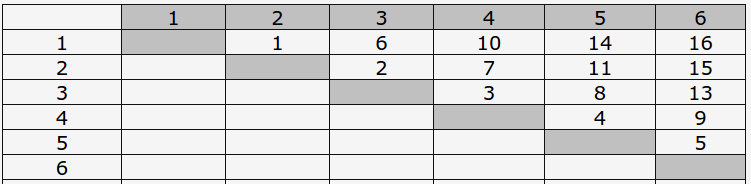
\includegraphics[width=8cm]{03/diagon}
\end{center}
Złożoność obliczeniowa wynika z:
\begin{itemize}
	\item dla każdej diagonali d ($n - 1$ różnych diagonali)
	\item dla każdej pozycji w~diagonali ($n - d$ pozycji)
	\item znajdź najlepszy podział ($j - i$ różnych wartości k, $ m(i,j) = \min\{m(i,k) + m(k+1, j) + p_{i-1} \cdot p_k \cdot p_j : i \le k < j\}$)
\end{itemize}

\subsection{Podsumowanie}
\begin{itemize}
	\item Liczba Catanala - \textbf{wykładnicza, $O(4^nn^\frac{-3}{2})$}
	\item Rekurencja (wielkość drzewa wywołań) - \textbf{wykładnicza, $O(2^{n-1})$}
	\item Programowanie dynamiczne - \textbf{potęgowa, $O(n^3)$ i $O(n^2)$}
	\item Szczegóły pod linkiem \href{http://edu.pjwstk.edu.pl/wyklady/asd/scb/asd14/main14_p2.html}{tutaj}
\end{itemize}




\section{Drzewie binarnym przeszukiwanie zgodnie z porządkiem inorder ma postać}

\vspace{0.4cm}
\noindent \textbf{Proponowana odpowiedź:} Zbadaj według kolejności: wierzchołek, lewe poddrzewo, prawe poddrzewo. \\

\noindent \textbf{Odpowiedź:} Zbadaj według kolejności: lewe poddrzewo, wierzchołek, prawe poddrzewo. \\

\noindent \textbf{Wyjaśnienie:}
\begin{figure}[h]	
	\centering	
	\subcaptionbox{Pre-order}
    {
		\begin{tikzpicture}[->,>=stealth',level/.style={sibling distance = 2cm/#1,level distance = 1.5cm},scale=0.6, transform shape]
		\node [treenode] {$1$}
		child { node [treenode] {$2$} }
		child { node [treenode] {$3$ } };
		\end{tikzpicture}
	}\qquad\qquad
    \subcaptionbox{In-order}
	{
		\begin{tikzpicture}[->,>=stealth',level/.style={sibling distance = 2cm/#1,level distance = 1.5cm},scale=0.6, transform shape]
		\node [treenode] {$2$}
		child { node [treenode] {$1$} }
		child { node [treenode] {$3$ } };
		\end{tikzpicture}
	} \qquad\qquad
	\subcaptionbox{Post-order}
	{
		\begin{tikzpicture}[->,>=stealth',level/.style={sibling distance = 2cm/#1,level distance = 1.5cm},scale=0.6, transform shape]
		\node [treenode] {$3$}
		child { node [treenode] {$1$} }
		child { node [treenode] {$2$ } };
		\end{tikzpicture}
	}
\end{figure} \\



\section{Złożoności}

\textbf{Zadanie o~rozmiarze $n$, realizowane pewnym algorytmem o~złożoności $f(n)$, zostało sprowadzone do~dwóch podzadań o~rozmiarze $\frac{n}{2}$ kazde oraz do~$n$~działań o~stałym czasie wykonania, zapewniających rozbicie i~scalenie zadania. Złożoność $f(n)$ wynosi:}\\
\textit{Przykładowa odp.) $f(n) = O(n\log{n})$}

\vspace{0.4cm}
\subsection{Wprowadzenie -- rodzaje złożoności}
\begin{description}
	\item[złożoność praktyczna] -- dla~podanego rozmiaru danych wyznacza dokładną liczbę elementarnych kroków potrzebnych do~wykonania danego algorytmu (oznaczenie \textbf{$T$})
	\item[złożoność teoretyczna] -- (klasa algorytmu) określa, jak silnie zależą od~siebie: rozmiar danych i~czas wykonania algorytmu - przy założeniu, że ten pierwszy wzrasta nieograniczenie (oznaczenie \textbf{$\Theta$})
	\item[notacja asymptotyczna] -- jeżeli $g(n)$ należy zarówno do $\Omega(f(n))$, jak i~do~$O(f(n))$, to~z~pewnością należy także do~$\Theta(f(n))$ 
	\begin{description}
		\item[dokładna] $ \Theta (f(n)) = \{ g(n): \exists_{c_1, c_2,n_0 > 0} \forall_{n \ge n_0} 0 \le c_1 f(n) \le g(n) \le c_2 f(n)  \} $
		\item[górne] $ O(f(n)) = \{ g(n): \exists_{c,n_0 > 0} \forall_{n \ge n_0} 0 \le g(n) \le c f(n)  \} $
		\item[dolne]$ \Omega (f(n)) = \{ g(n): \exists_{c,n_0 > 0} \forall_{n \ge n_0} 0 \le  c f(n) \le g(n) \} $
	\end{description}
\end{description}
\subsection{Rozwiązanie}
Korzystamy z~twierdzenia o~rekurencji uniwersalnej:
Niech $a \ge 1$ i $b > 1$ będą stałymi, $f(n)$ dowolną funkcją, zaś $T(n)$ zdefiniowane dla~nieujemnych liczb całkowitych poprzez rekurencję:
$$T(n) = aT(\frac{n}{b}) + f(n)$$
Wówczas $T(n)$ możemy asymptotycznie oszacować w~następujący sposób:
\begin{enumerate}
	\item Jeśli $f(n) = O(n^{\log_b {(a -\epsilon)}})$ dla pewnej stałej $\epsilon > 0$, to $T(n) = \Theta(n^{\log_b a})$
	\item Jeśli $f(n) = \Theta(n^{\log_b {a}})$, to $T(n) = \Theta(n^{\log_b a} \log n)$
	\item Jeśli $f(n) = \Omega(n^{\log_b {(a + \epsilon)}})$ dla pewnej stałej $\epsilon > 0$, to $T(n) = \Theta(f(n))$
\end{enumerate}

Oznaczenia mogą być trochę mylące. Niech $f$ z~treście pytania będzie oznaczone $T$. Wtedy $T(n) = 2T(\frac{n}{2}) + n$. Funkcja $f$ z~twierdzenia to~$n$, $a = 2$, $b = 2$, $\log_2 2 = 1 $, więc spełniony jest podpunkt 2. Odpowiedź to~\textbf{$\Theta(n\log n)$} (a~więc także $O(n\log n)$ i~$\Omega (n\log n)$).





\section{Dany jest graf skierowany G = (V,E), gdzie V =\{1,2,3,4,5,6\}, E = \{(1,2), (1,3), (2,4), (2,5), (4,5), (5,1), (3,5), (3,6)\}. Jeśli graf G przeszukujemy w głąb poczynając od wierzchołka 1 to}

\vspace{0.4cm}
\noindent \textbf{Proponowana odpowiedź:} Krawędź (2,5) może być krawędzią drzewową (w zależności od realizacji algorytmu) \\

\noindent \textbf{Odpowiedź:}  
\begin{itemize}
	\item Możliwa kolejność odwiedzonych wierzchołków: $1, 2, 4, 5, 3, 6$
	\item Krawędzie drzewowe: $(1, 2), (2, 4), (4, 5), (1, 3), (3, 6)$.
	\item Krawędzie wprzód: $(2, 5), (3, 5)$
	\item Krawędzie powrotne: $(5, 1)$
	\item Krawędzie $(2,5), (3, 5)$ może być drzewowe, w zależności od realizacji algorytmu 
	\item Krawędź $(4, 5)$ może być wprzód, w zależności od realizacji algorytmu 
\end{itemize}

\noindent \textbf{Wyjaśnienie:}
Zbiór wszystkich drzew przeszukiwania w głąb - które zostały utworzone podczas przechodzenia po grafie - nazywamy lasem przeszukiwania w głąb.
Przechodząc pod grafie możemy dokonać klasyfikacji krawędzi na:
\begin{itemize}
	\item krawędzie drzewowe - są to krawędzie których zbadanie powoduje odkrycie nowego wierzchołka
	\item krawędzie powrotne - są to krawędzie łączące wierzchołek z przodkiem
	\item krawędzie w przód - są to krawędzie niedrzewowe, łączące wierzchołek z potomkiem
	\item krawędzie poprzeczne - wszystkie inne krawędzie
\end{itemize}  


\section{Zgadywanka}
\textbf{Które stwierdzenia sposród poniższych są prawdziwe (haha.)}\\
\textit{przykładowa odp.) Algorytm Dijkstry ma własność optymalnej podstruktury,}

\vspace{0.4cm}

Przykładowa odpowiedź jest prawdziwa, bo ``The subpath of~any~shortest path is~itself a~shortest path'', a~problem z~optymalną podstrukturą to~taki, którego optymalne rozwiązanie może być~efektywnie skonstruowane z~optymalnych rozwiązań podproblemów. Zwykle własność optymalnej podstruktury oznacza, że problem może być rozwiązany algorytmem zachłannym lub dynamicznym.




\section{Dana jest procedura xxx. Przyjmij konwencję, że np. zapis AAABCC oznacza trzykrotne wykonanie instrukcji A, po czym następuje wykonanie instrukcji B a następnie dwukrotnie instrukcji C. Następujące sekwencje instrukcji mogą być wynikami wywołania powyższej procedury}
\begin{lstlisting}
Proc(n) {
	if (warunek(x)) then {
		A(x);
		Proc(f(n));
		B(x);
	} else
		C(x);
}
\end{lstlisting}

\vspace{0.4cm}
\noindent \textbf{Proponowana odpowiedź:} AAACCCBBB \\ 

\noindent \textbf{Odpowiedź:} $A^xCB^x, x \ge 0$ \\

\noindent \textbf{Wyjaśnienie:}
Funkcja Proc jest rekurencyjnie wywoływana pomiędzy wywołaniem A i B. W przypadku kiedy warunek jest spełniony, Proc rozpoczyna się od wywołania funkcji A, następnie rekurencyjnie wywołuje siebie, odkładając wywołanie funkcji B "na później". Będzie to następować tak długo jak warunek jest spełniony. W momencie kiedy warunek będzie niespełniony nastąpi wywołanie funkcji C oraz pozostałe wywołania funkcji B odłożone na stosie wywołań. \\

\section{BST}
\textbf{Graf $G = (V, E)$ jest drzewem BST, przy czym $V = \{15, 21, 23, 29, 31, 38, 40, 61, 96, 98\}$, $E = \{(21, 15),(21, 23),(29, 21),(29, 31),(38, 29),(38, 96),(96, 40),(96, 98),(40, 61)\}$.}\\
\textit{przykładowa odp.) W wyniku przeszukiwania postorder wierzchołki zostaną odwiedzone w następującej kolejności: 15, 23, 21, 29, 31, 61, 40, 98, 96, 38.}

\vspace{0.4cm}

Na~podstawie krawędzie łatwo można narysować taki graf

\begin{center}
	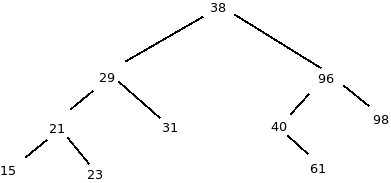
\includegraphics[width=8cm]{03/bst}
\end{center}

Mamy trzy możliwe rodzaje przejść Depth First:
\begin{itemize}
	\item preorder (vlr) 
	\begin{lstlisting}
	preorder(node)
	if node == null then return
	visit(node)
	preorder(node.left) 
	preorder(node.right)
	\end{lstlisting}
	- wynik:  38, 29, 21, 15, 23, 31, 96, 40, 61, 98
	\item inorder (lvr) 
	\begin{lstlisting}
	inorder(node)
	if node == null then return
	inorder(node.left)
	visit(node)
	inorder(node.right)
	\end{lstlisting}
	- wynik: 15, 21, 23, 29, 31, 38, 40, 61, 96, 98
	\item postorder (lrv)
	\begin{lstlisting}
	postorder(node)
	if node == null then return
	postorder(node.left)
	postorder(node.right)
	visit(node)
	\end{lstlisting}
	- wynik: 15, 23, 21, 31, 29, 61, 40, 98, 96, 38
\end{itemize}

Możliwe jest także przejście Breadth-First (odwiedzany jest każdy węzeł na~poziomie przed zejściem na~kolejny poziom). Wynik: 38, 29, 96, 21, 31, 40, 98, 15, 23, 61.\\
Przykładowa odpowiedź jest nieprawdziwa.


\section{Niech $p=(x_1, y_1)$, $q=(x_2, y_2)$, $r=(x_3, y_3)$ oraz $det(p, q, r)$, oznacza wyznacznik macierzy}
\noindent $x_1 \quad y_1 \quad 1$ \\
$x_2 \quad y_2 \quad 1$ \\
$x_3 \quad y_3 \quad 1$


\vspace{0.4cm}
\noindent \textbf{Proponowana odpowiedź:} Jeśli $det(p, q, r) = 0$ to punkt $r$ leży na prostej wyznaczonej przez punkty p i q \\ 

\noindent \textbf{Odpowiedź:}
\begin{itemize}
	\item Jeśli $det(p, q, r) > 0$ to punkt $r$ leży po lewej stronie wektora p $\rightarrow$ q
	\item Jeśli $det(p, q, r) = 0$ to punkt $r$ leży na prostej wyznaczonej przez punkty p i q
	\item Jeśli $det(p, q, r) < 0$ to punkt $r$ leży po prawej stronie wektora p $\rightarrow$ q
	\item Jeśli $sgn(det(p, q, p_1)) = sgn(det(p,q, p_2))$, punkty $p_1$ i $p_2$ leżą po tej samej stronie prostej $p - q$
\end{itemize}

\noindent \textbf{Wyjaśnienie:}
Algorytmy geometryczne. Wzięte z wykładów prof. Bieleckiego.


\section{Problem przynależności punktu do wielokąta}

\textbf{Danych jest n~punktów wyznaczających wielobok o~n~bokach.}\\
\textit{przykładowa odp.) Istnieje algorytm o~złozoności $O(\log n)$ sprawdzający, czy~zadany punkt nalezy do~wnętrza wieloboku.}

\vspace{0.4cm}

\subsection{Problem}
No~dobra, ogarnijmy o~co~chodzi w~zagadnieniu. Będzie fajnie.

Dla danego punktu p~sprawdź, czy~p~znajduje się~wewnątrz, czy~na~zewnątrz n-kąta reprezentowanego przez ciąg kolejnych krawędzi.
\subsection{Zliczanie przecięć krawędzi}

\begin{lstlisting}
poprowadz z p pionowa polprosta l;
k:=0; 
wybierz bok wielokata f;
repeat
if  l przecina f
then k:=k+1;
f:=kolejny bok wielokata;
until wszystkie boki wielokata zostaly zbadane; 
if  k parzyste then p jest na zewnatrz
else p jest wewnatrz;
\end{lstlisting}

Widzimy, że~złożoność algorytmu to~$O(n)$. Algorytm nie~bierze pod~uwagę przypadków szczególnych (półprosta zawiera wierzchołek/krawędź) -- ich~uwzględnienie nie~zmienia złożoności obliczeniowej.

Ok, dalej: lokalizacja punktu względem wielokąta wypukłego. Problem prostszy.

Definicja: Górnym (dolnym) łańcuchem wielokąta wypukłego nazywamy ciąg jego krawędzi między skrajnie lewym a~skrajnie prawym wierzchołkiem wielokąta odwiedzanych zgodnie z~ruchem wskazówek zegara (przeciwnie do~ruchu wskazówek zegara).
\begin{center}
	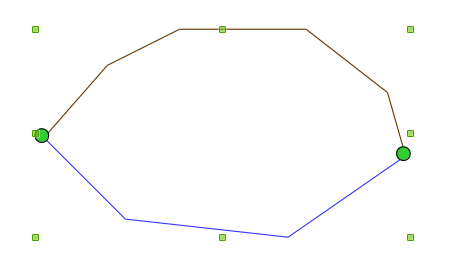
\includegraphics[width=4cm]{03/lancuch}
\end{center}

Półprosta poprowadzona z~danego punktu przecina każdy z~łańcuchów wielokąta wypukłego w~co~najwyżej jednym punkcie (jeśli przetnie dwa razy, jest poza; jeśli raz, jest w~środku).

Wyszukiwanie przecięcia:
krawędzie łuku mamy w~tablicy, zaczynamy od~środkowego elementu i~w~zależności, czy~półprota jest po~prawej czy~po~lewej idziemy w~odpowiednią stronę. Jest to~przeszukiwanie drzewa, a~więc $O(\log n)$.

Dla uogólnienia problemu do~przestrzeni \textbf{trójwymiarowej} istnieje analogiczny algorytm o~złożoności $O(n)$.

\subsection{Zliczanie zakrętów}
Winding Number Algorithm -- zliczamy ile razy krawędzie ``skręcają'' w~lewo (+1) i~ile w~prawo (-1), jeśli wyjdzie 0 mamy pełny obrót (jesteśmy w~środku).

Jeśli jesteśmy po~lewej stronie krawędzi skierowanej w~lewo, zakręt w~lewo.\\
Jeśli jesteśmy po~prawej stronie krawędzi skierowanej w~prawo (patrząc zgodnie ze~strzałką), zakręt w~prawo.
\begin{center}
	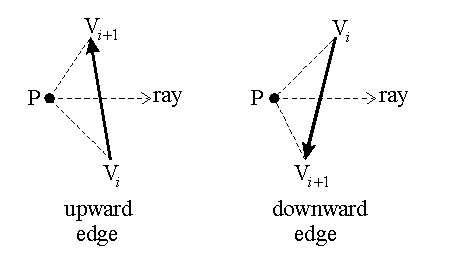
\includegraphics[width=6cm]{03/uede}
\end{center}

\begin{lstlisting}
wn_PnPoly( Point P, Point V[], int n )
{
int    wn = 0;    // the  winding number counter

// loop through all edges of the polygon
for (each edge E[i]:V[i]V[i+1] of the polygon) {
if (E[i] crosses upward ala Rule #1)  {
if (P is  strictly left of E[i])    // Rule #4
++wn;   // a valid up intersect right of P.x
}
else
if (E[i] crosses downward ala Rule  #2) {
if (P is  strictly right of E[i])   // Rule #4
--wn;   // a valid down intersect right of P.x
}
}
return wn;    // =0 <=> P is outside the polygon

}
\end{lstlisting}

Złożoność $O(n)$.
\subsection{Podsumowanie}
\begin{itemize}
	\item dla wielokąta w~2D: $O(n)$
	\item dla wielokąta wypukłego w~2D: $O(\log n)$
	\item dla wielokąta w~3D: $O(n)$
	\item dla wielokąta w~2D istnieje jeszcze algorytm ``Winding Number'' (na~polski indeks punktu względem krzywej) o~złożoności $O(n)$.
\end{itemize}




\section{Graf dynamiczny, którego maksymalnej liczby wierzchołków i krawędzi w trakcie wykonywania algorytmu nie potrafimy z góry oszacować powinien być reprezentowany jako}


\vspace{0.4cm}
\noindent \textbf{Proponowana odpowiedź:} Lista list \\ 

\noindent \textbf{Odpowiedź:} Lista sąsiedztwa zaimplementowana jako lista list. \\

\noindent \textbf{Wyjaśnienie:}
Lista sąsiedztwa jest listą list. Każdy element głównej listy odpowiada jednemu wierzchołkowi $u$ opisywanego grafu. W liście przechowywane są wskaźnili na listy zawierające wierzchołki $v_x$ sąsiednie do $u$. Operacje w większości wykonują się wolniej niż w przypadku macierzy sąsiedztwa. Zaletą jest duża elastyczność w przypadku zmiany ilości wierzchołków oraz mniejsza złożoność pamięciowa, liniowa względem krawędzi.



\section{Problem komiwojażera}

\textbf{Dla problemu komiwojażera algorytm pozwalający wyznaczyć rozwiązanie optymalne:}\\
\textit{przykładowa odp.) istnieje i ma złozoność wykładniczą}

\vspace{0.4cm}


\subsection{Problem}
Dany pełny graf n-wierzchołkowy z~nieujemnymi wagami na~krawędziach. Znaleźć cykl Hamiltona (cykl, w~którym każdy wierzchołek odwiedzony jest dokładnie raz) o~najmniejszej wadze (tzn. sumie wag krawędzi).

\noindent Problem należy do~klasy NP-hard (NP-trudnych).\\
Problem \textbf{decyzyjny} komiwojażera należy do~klasy NP-complete (NP-zupełnych).\\
Problem \textbf{metryczny} komiwojażera należy do~klasy NP-complete (NP-zupełnych). (spełniona jest nierówność trójkąta dla każdej trójki wierzchołków).\\

\subsection{Algortymy}
\begin{itemize}
	\item istnieje algorytm o~złożoności wykładniczej względem liczby wierzchołków wyznaczający rozwiązanie optymalne
	\item dla metrycznego problemu komiwojażera istnieje \textbf{algorytm 2-aproksymacyjny} o~złożoności \textbf{wielomianowej} (znalezione rozwiązanie jest lepsze niż drukrotność optymalnego)
	\item dla metrycznego problemu komiwojażera istnieje \textbf{algorytm $\frac{3}{2}$-aproksymacyjny} o~złożoności \textbf{wielomianowej} - jak na~razie najlepszy stopień przybliżenia rozwiązania
	\item dla klasycznego algorytmu komiwojażera nie istnieje żaden algorytm aproksymacyjny (o~ile P != NP, brak dowodu)
\end{itemize}

Algorytm 2-apryksymacyjny: (chyba tutaj niepotrzebny, dlatego nie rozwijany zanadto)
\begin{enumerate}
	\item Znajdź minimalne drzewo spinające T (algorytm Prima, minimalne drzewo rozpinające -- algorytm oblicza podzbiór E' zbioru krawędzi E, dla którego graf nadal pozostaje spójny, ale suma kosztów wszystkich krawędzi zbioru E' jest najmniejsza możliwa)//
	w~skrócie wywalamy wszystkie krawędzie tak, żeby można było dostać się~z~każdego wierzchołka do~innego wierzchołka, i~żeby suma wag krawędzi była najmniejsza; złożoność algorytmu zależy od~zastosowanej struktury danych.
	\item Dodaj krawędzie tak aby stopień każdego wierzchołka był parzysty (stopień = liczba wychodzących krawędzi)
	\item Otrzymany graf  X jest eulerowski (da~się w~nim skonstruować cykl Eulera, czyli cykl, który przechodzi przez każdą jego krawędź dokładnie raz i~wraca do punktu wyjściowego)
	\item Przekształć cykl Eulera w cykl Hamiltona
\end{enumerate}


\section{Głębokość rekurencji dla ciągu Fibonacciego zaimplementowanego rekurencyjnie zgodnie z arytmetyczną definicją rekurenycjną wynosi}

\vspace{0.4cm}
\noindent \textbf{Proponowana odpowiedź:} $O(n^4)$ \\ 

\noindent \textbf{Odpowiedź:} $O(2^n)$ \\

\noindent \textbf{Wyjaśnienie:}
$T(n) = T(n-1) + T(n-2) + c \leq 2T(n-1) + c = 2(2T(n-2) + c) + c = 2^2T(n-2) + 2c + 2^0c =...= 2^nT(0) + 2^{n-1}c + ... + 2c + 2^0c = c(2^n-1)$ \\


\section{Kursorowa implementacja listy}
\textbf{Kursorowa implementacja listy jest strukturą}\\
\textit{przykładowa odp.) rekordową}

\vspace{0.4cm}


\subsection{Kursorowa implementacja listy}
W~językach nie posiadających referencji ani wskaźników nie~istnieje możliwość klasycznej implementacji listy. Z~tego powodu stosuje się~tablicę \textbf{rekordów}. Każdy rekord przechowuje wartość elementu oraz indeks wskazujący, na~którym miejscu w~tablicy znajduje się~kolejny element (w~przypadku listy podwójnie wiązanej, zarówno następny jak i~poprzedni).

\begin{lstlisting}
record Entry {
integer next; // index of next entry in array
integer prev; // previous entry (if double-linked)
string name;
real balance;
}
\end{lstlisting}
Dodatkowo konieczne jest przechowywanie osobno indeksu pierwszego elementu listy.

``W~celu sprawniejszego znajdowania miejsca wolnego w~tablicy, można wszystkie wolne miejsca powiązać w~tzw. \textbf{listę pamięci wolnej}, w~której pierwszy element jest przechowywany przez  globalną zmienną o~nazwie np.~firstfree'' A. Bielecki 

\subsection{Odpowiedź}
Tak, jest strukturą \textbf{rekordową}. Jest też \textbf{tablicową} (tak?)

\section{Problem chińskiego listonosza polega na}
\noindent \textbf{Proponowana odpowiedź:} Znalezieniu najkrótszej drogi zamkniętej zawierającej wszystkie wierzchołki grafu. \\

\noindent \textbf{Odpowiedź}:  Znalezieniu najkrótszej drogi zamkniętej zawierającej wszystkie \textbf{krawędzie} grafu. \\

\noindent \textbf{Wyjaśnienie}:
Rozważmy graf, którego krawędzie odpowiadają ulicom w rejonie, obsługiowanym przez listonosza. Wierzchołki to po prostu skrzyżowania ulic. Krawędziom nadajemy wagi, które oznaczają odległości między dwoma skrzyżowaniami. Znalezienie możliwie najkrótszej drogi, którą musi przejść listonosz sprowadza sie do znalezienia w tym grafie drogio minimalnej sumie wag krawędzi, która przechodzi przez każdą krawędź co najmniej raz. Jeśli dany graf posiada cykl Eulera, to istnieje taka droga, która zaczyna i konczy sie w tym samym punkcie i wymaga przejścia po każdej ulicy dokładnie raz. Problem ma zawsze rozwiązanie jeżeli graf jest spójny. 